\clearpage
\subsection*{PPL de maximizare – producție}
\paragraph{}
Compania \textbf{Chevrolet} dorește să obțină un venit maxim în urma producției de mașini. Modelele pe care aceasta companie le produce sunt Aveo, Colorado, Camaro, Suburban. Resursa limitată pentru producția acestor mașini este timpul pentru fiecare proces, este nevoie de 4 procese pentru a face o mașină. Datele problemei sunt date în tabelul de mai jos.

\paragraph{}
\begin{figure}[h]
\begin{center}
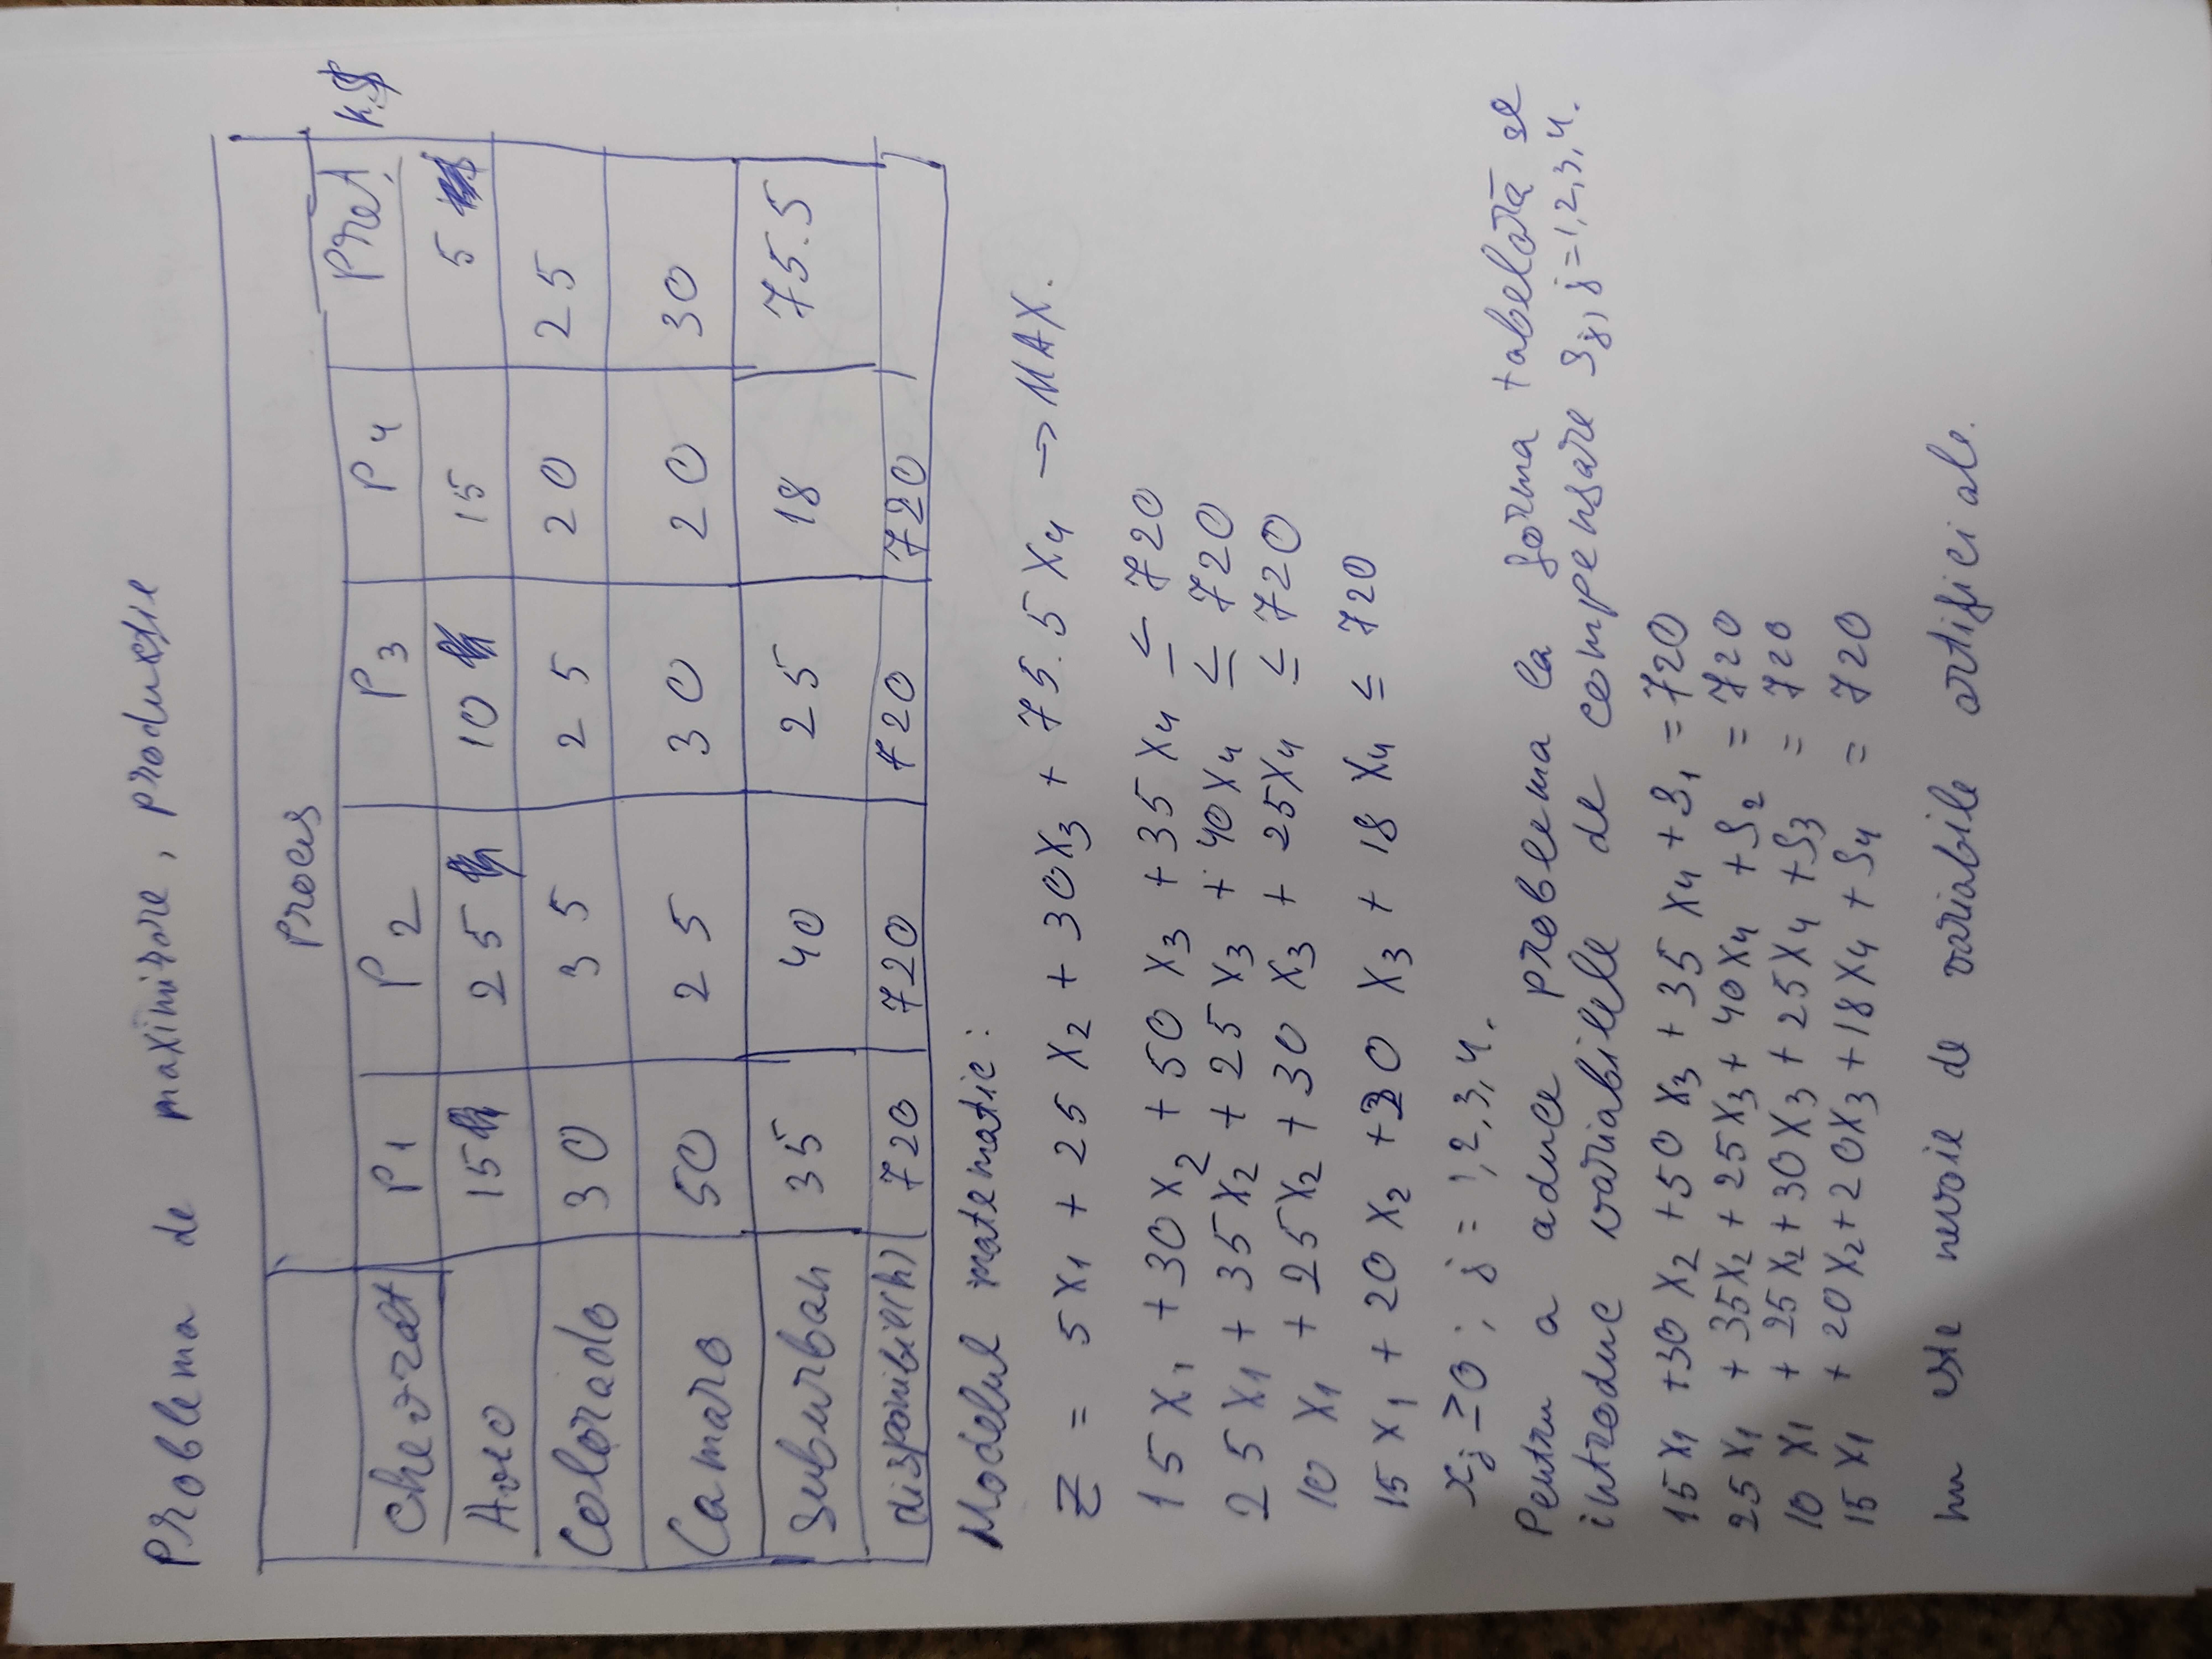
\includegraphics[width=22cm, angle =-90]{1}
\caption{Datele problemei și modelul matematic} 
\label{fig:1}
\end{center}
\end{figure}

\paragraph{}
\begin{figure}[h]
\begin{center}
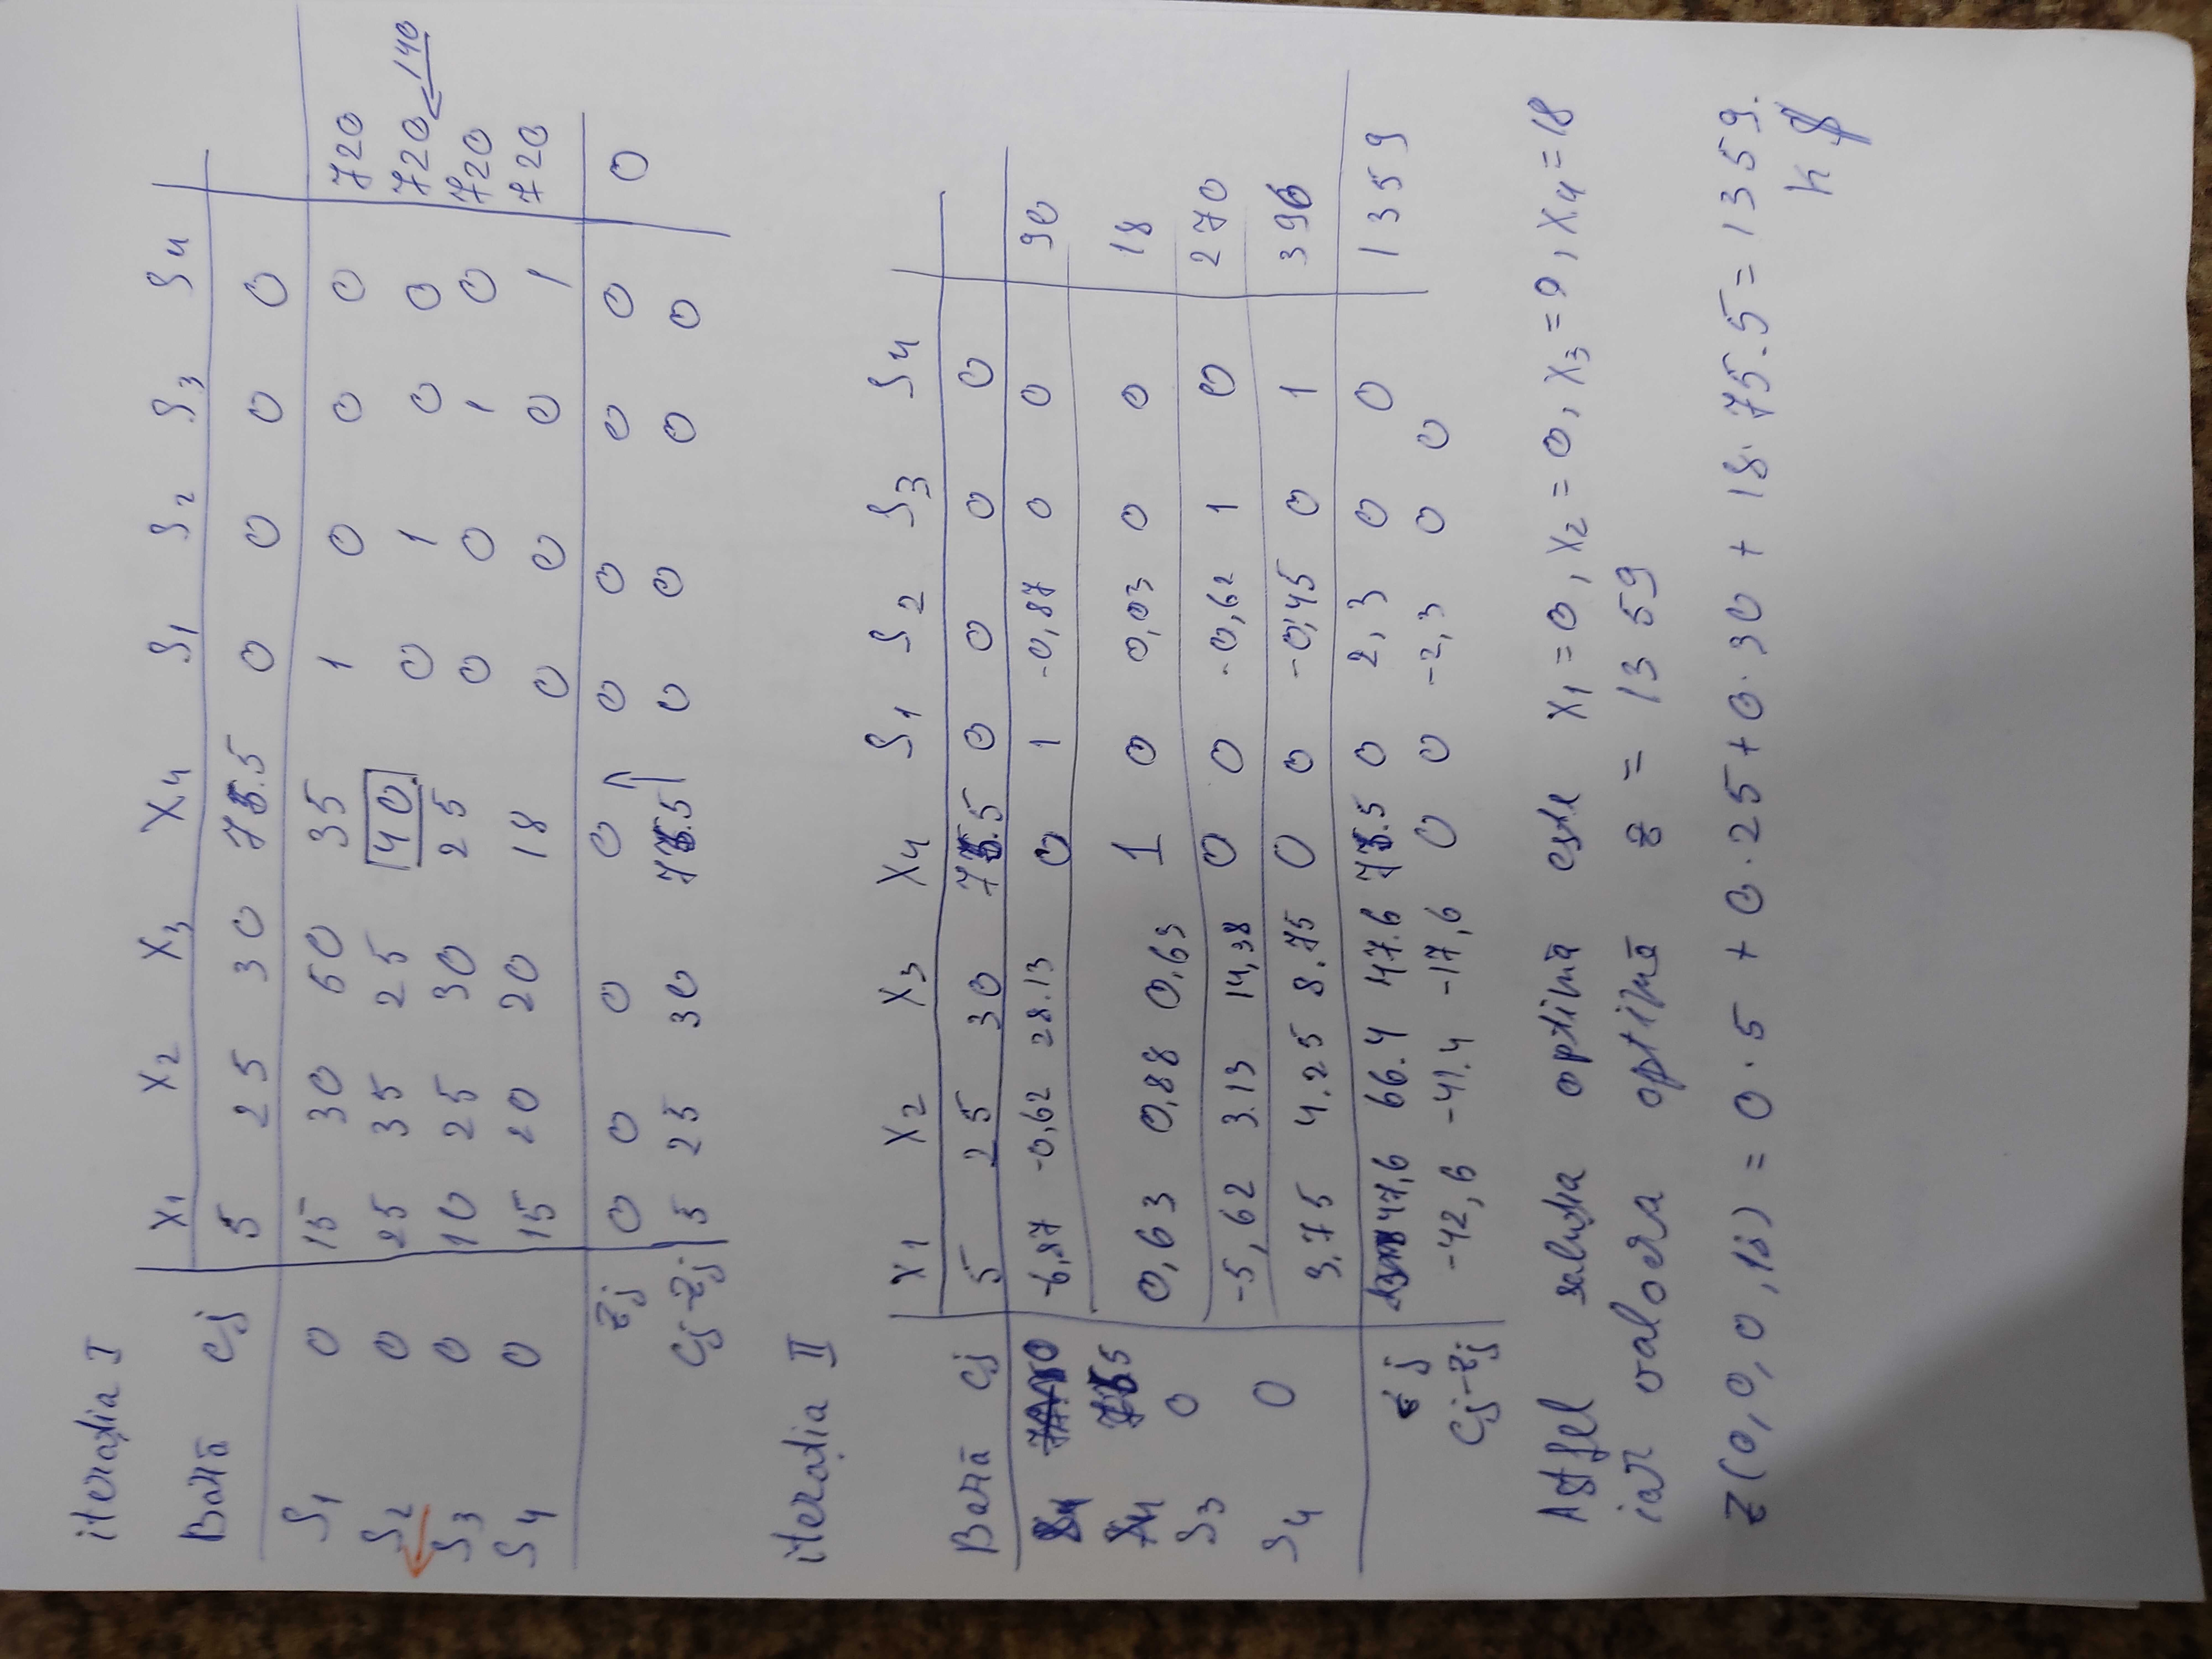
\includegraphics[width=22cm, angle =-90]{2}
\caption{Metoda simplex} 
\label{fig:2}
\end{center}
\end{figure}

